\documentclass[12pt]{article}
\usepackage{geometry}
\geometry{a4paper, margin=2cm}
\usepackage{longtable}
\usepackage{titlesec}
\usepackage{fontspec}
\usepackage{hyperref}
\usepackage{graphicx}
\usepackage{float}
\usepackage{listings}
\usepackage{color}
\usepackage{pdfpages} % подключаем пакет для работы с PDF

%\setmainlanguage{russian} % если ваш основной язык русский
\definecolor{codegreen}{rgb}{0,0.6,0}
\definecolor{codegray}{rgb}{0.5,0.5,0.5}
\definecolor{codepurple}{rgb}{0.58,0,0.82}
\definecolor{backcolour}{rgb}{0.95,0.95,0.92}
\lstdefinestyle{mystyle}{
    backgroundcolor=\color{backcolour},
    commentstyle=\color{codegreen},
    keywordstyle=\color{magenta},
    numberstyle=\tiny\color{codegray},
    stringstyle=\color{codepurple},
    basicstyle=\ttfamily\footnotesize,
    breakatwhitespace=false,
    breaklines=true,
    captionpos=b,
    keepspaces=true,
    numbers=left,
    numbersep=5pt,
    showspaces=false,
    showstringspaces=false,
    showtabs=false,
    tabsize=2,
    frame=single,
    escapeinside=``,
}

\lstset{style=mystyle}


\setmainfont{Times New Roman}
\titleformat{\section}{\normalfont\Large\bfseries}{\thesection}{1em}{}

\title{База знаний по проектному управлению и управлению рисками}
\author{}
\date{}

\begin{document}

\maketitle

\section*{Введение}
В условиях высокой сложности и многозадачности крупных проектов, особенно в промышленности, возрастает нагрузка на управленческий персонал. Целью данной работы является создание концепции интеллектуального помощника, который бы автоматизировал рутинные функции анализа, мониторинга и поддержки принятия решений, облегчая работу руководства проекта. В основе решения лежит база знаний, сформированная из открытых источников крупнейших российских компаний (СИБУР, РОСАТОМ, РУСАЛ и др.).

\section{Цель и задачи разработки помощника}
\begin{itemize}
    \item Повышение эффективности управления проектами за счёт автоматизации рутинных решений.
    \item Поддержка оценки рисков и отклонений по ключевым метрикам.
    \item Ведение базы знаний на основе лучших корпоративных практик.
    \item Поддержка сценарного анализа и генерации альтернативных решений.
\end{itemize}

\section{Анализ открытых данных компаний}
\begin{longtable}{|c|p{3.5cm}|p{3.5cm}|p{3.5cm}|p{4.5cm}|}
    \hline
    \textbf{№} & \textbf{Что искать} & \textbf{Ключевые слова} & \textbf{Что выписывать} & \textbf{Зачем это помощнику} \\
    \hline
    1 & Управление проектами & инвестиционные проекты, Value Engineering & Модель управления, контроль, роли & Основа понимания хода проекта \\
    \hline
    2 & Классификация рисков & риск-менеджмент, сценарный анализ & Типы рисков, меры реагирования & Чтобы оценивать и предотвращать риски \\
    \hline
    3 & ИИ и цифровизация & цифровизация, ИИ, предиктивная аналитика & Где применяется ИИ & Для генерации сценариев и RAG \\
    \hline
    4 & ESG и устойчивость & ESG, декарбонизация, углеродный след & Стратегии и риски ESG & Чтобы учитывать внешние ограничения \\
    \hline
    5 & Органы управления & проектный офис, совет директоров & Кто за что отвечает & Помощник может знать, кому сообщить \\
    \hline
    6 & Метрики и KPI & эффективность, результативность & Сроки, бюджеты, выработка & Для выявления отклонений \\
    \hline
    7 & Контроль и аудит & мониторинг, контроль исполнения & Механизмы контроля & Помощник может следить за выполнением \\
    \hline
    8 & Стандарты и методы & регламенты, шкалы оценки & Внутренние классификаторы & Можно использовать для обучения модели \\
    \hline
    \end{longtable}
\subsection{СИБУР}
    \begin{longtable}{|p{4.5cm}|p{6cm}|p{4.5cm}|}
        \hline
        \textbf{Раздел / Источник} & \textbf{Выдержка / Ключевая информация} & \textbf{Комментарий} \\
        \hline
        \endfirsthead
        \hline
        \textbf{Раздел / Источник} & \textbf{Выдержка / Ключевая информация} & \textbf{Комментарий} \\
        \hline
        \endhead
        
        \textbf{Перспективы развития и цифровизация} &
        «СИБУР активно вовлечен в НИОКР… моделирование полимеров и их свойств с применением ИИ» &
        ИИ применяется в исследованиях и цифровых экспериментах — фундамент для RAG и сценарного анализа. \\
        \hline
        
        \textbf{Инвестиционные проекты} &
        «Укрепляется функция проектного управления… Value Engineering… база знаний по реализуемым проектам» &
        Развита методология проектного контроля, включая предиктивный анализ и накопление опыта. \\
        \hline
        
        \textbf{Раздел “Ключевые риски”} &
        «Риски: макроэкономический, геополитический, логистический, информационный, ESG, инвестиционный» &
        Даётся классификация рисков + меры управления, сценарный анализ, диверсификация, контроль подрядчиков. \\
        \hline
        
        \textbf{Раздел об устойчивом развитии} &
        «Обновлена стратегия устойчивого развития… ESG-рейтинг на уровне AAA.esg…» &
        Интеграция ESG и климатических рисков в KPI проектов. Оценка и декарбонизация как часть стратегических проектов. \\
        \hline
        
        \end{longtable}
        
    
% Здесь будет таблица с выдержками из годового отчёта (уже почти готова)
%\input{tables/sibur.tex} % или вставим прямо вручную позже

\subsection{РОСАТОМ}

\begin{longtable}{|p{4.5cm}|p{6cm}|p{4.5cm}|}
\hline
\textbf{Раздел / Источник} & \textbf{Выдержка / Ключевая информация} & \textbf{Комментарий} \\
\hline
\endfirsthead
\hline
\textbf{Раздел / Источник} & \textbf{Выдержка / Ключевая информация} & \textbf{Комментарий} \\
\hline
\endhead

\textbf{Нормативные документы «Управление рисками при обращении с ОЯТ и РАО»} (Росатом) & 
«Оценка технологического риска включает расчет финансовых потерь и выгод… интегральная оценка значимости» & 
Формализованный подход с выручкой, вероятностью и последствиями. \\
\hline

\textbf{Отчёт по цифровизации} («Русатом‑Цифровые решения») & 
«Созданы … структуры по внутренней цифровизации атомной отрасли» & 
Наличие отдельного подразделения для цифровых проектов. \\
\hline

\textbf{ESG‑отчет 2023} & 
«Подтверждён уровень „А“ в ESG‑рейтинге … полностью управляет ESG‑рисками» & 
Корпоративная зрелость ESG-управления на высоком уровне. \\
\hline

\textbf{Общий публичный отчёт 2023} & 
«В 2023 проходили слёты лидеров безопасности … комитет — часть системы управления» & 
Системный подход к культуре безопасности. \\
\hline

\textbf{Инфраструктурные цифровые проекты} & 
«Строительство ЦОД рядом с Калининской АЭС … в рамках цифровой экономики» & 
Примеры больших цифровых проектов, обеспечение ИТ‑инфраструктуры. \\
\hline

\end{longtable}

% Добавим позже

\subsection{РУСАЛ}
\begin{longtable}{|p{4.5cm}|p{6cm}|p{4.5cm}|}
    \hline
    \textbf{Раздел / Источник} & \textbf{Выдержка / Ключевая информация} & \textbf{Комментарий} \\
    \hline
    \endfirsthead
    \hline
    \textbf{Раздел / Источник} & \textbf{Выдержка / Ключевая информация} & \textbf{Комментарий} \\
    \hline
    \endhead
    
    \textbf{Sustainability Report 2023} &
    «специфические выбросы парниковых газов снижены на 6.7 \%, удельные выбросы в электролизе — на 11.4 \%» &
    Отражено снижение климатических рисков через количественные KPI. \\
    \hline
    
    \textbf{Управление климатическими рисками} &
    «Оценка климатических рисков выполнена по трём сценариям SSP 126, 245, 585 с оценкой влияний» &
    Используется сценарный анализ — готовый кейс для моделирования помощником. \\
    \hline
    
    \textbf{CDP / ESG-пресс-релиз 2025} &
    «RUSAL получил рейтинг CDP «A−»… оценивает и управляет климатическими рисками с 2015 года» &
    Усиленная ESG-практика с признанием международных стандартов. \\
    \hline
    
    \textbf{AI для контроля плавки} (июль 2025) &
    «RUSAL внедряет искусственный интеллект для мониторинга технологии плавления — ИИ снижает риск низкого качества сплава» &
    Конкретный пример ИИ‑проекта для контроля процессов и качества. \\
    \hline
    
    \textbf{Устойчивое развитие — сайт компании} &
    «Горизонт стратегий до 2035 г.— цель: углеродная нейтральность, эфффект декаплинга» &
    Долгосрочная ESG-стратегия — база для стратегического мониторинга в помощнике. \\
    \hline
    
    \end{longtable}
% Добавим позже

\section{Гипотезы для мониторинга проекта}

Помощник использует набор формализованных правил для оценки состояния проекта. Ниже представлены ключевые гипотезы, основанные на типовых отклонениях и лучших практиках управления.

\begin{longtable}{|p{1.2cm}|p{5.5cm}|p{8cm}|}
\hline
\textbf{ID} & \textbf{Гипотеза} & \textbf{Комментарий / Основание} \\
\hline
\endfirsthead
\hline
\textbf{ID} & \textbf{Гипотеза} & \textbf{Комментарий / Основание} \\
\hline
\endhead

H1 & Если отклонение по срокам задач > 15\% от базового графика, то проект попадает в жёлтую зону риска. & Используется в системе оценки инвестиционных проектов (СИБУР, ROSATOM). \\
\hline

H2 & Если бюджет превышен более чем на 10\% — пометить как “рисковое отклонение” и инициировать повторную оценку. & Типовой предел управления CAPEX/контроля затрат. \\
\hline

H3 & Если в течение 2 недель подряд фиксируются отклонения по 3 и более KPI — система предупреждает руководителя. & Используется для выявления скрытых отклонений (набор слабых сигналов). \\
\hline

H4 & Если уровень ESG-показателей падает ниже внутреннего порога (например, выбросы СО₂ выросли > 5\%), проект помечается как “критичный по устойчивости”. & На базе данных из отчётов РУСАЛ и РОСАТОМ. \\
\hline

H5 & Если подрядчик пропускает более 1 контрольной точки подряд — вывести рекомендацию по замене. & Стратегия управления подрядчиками у СИБУРа. \\
\hline

H6 & Если вероятность наступления любого риска > 70\%, активировать сценарный анализ. & Сценарные расчёты SSP / WEF risk maps применимы. \\
\hline

H7 & Если зафиксирован системный сбой в ИИ-мониторинге (например, в технологическом контроле), приостановить операции и инициировать ручную проверку. & По аналогии с ИИ-кейсом РУСАЛ (контроль плавки). \\
\hline

\end{longtable}

\section{Концепция сценарного моделирования реализации проекта}

Сценарное моделирование используется для анализа потенциальных отклонений и выработки решений в условиях неопределённости. Интеллектуальный помощник использует данные о текущем состоянии проекта, вероятностях рисков и внешних ограничениях для генерации альтернативных графиков и рекомендаций.

\subsection{Входные данные для моделирования}
\begin{itemize}
    \item Базовый график проекта (этапы, сроки, зависимости);
    \item Структура рисков (вероятности, влияние, тип);
    \item Текущие метрики: отклонение по срокам и стоимости;
    \item ESG‑ограничения и внешние сценарии (например, SSP 1–2.6, 2–4.5, 5–8.5);
    \item Данные о подрядчиках и их надёжности;
    \item Пользовательские параметры: приоритеты (стоимость/время/качество).
\end{itemize}

\subsection{Выходные сценарии}
\begin{itemize}
    \item Альтернативные графики реализации (перестановка задач, замена подрядчиков);
    \item Вероятностная оценка завершения проекта в срок и в пределах бюджета;
    \item Рекомендации по снижению рисков;
    \item Режим «что если» (What-If) — анализ ключевых решений.
\end{itemize}

\subsection{Алгоритм сценарного анализа (концептуально)}
\begin{enumerate}
    \item Получить текущие данные проекта;
    \item Проверить срабатывание гипотез мониторинга;
    \item При выявлении угроз — построить дерево сценариев:
    \begin{itemize}
        \item Ветвление по типу риска (время, ресурсы, регуляторика);
        \item Варианты реакции: ускорение, перераспределение, замена подрядчиков;
        \item Расчёт вероятности выполнения сценария.
    \end{itemize}
    \item Предложить пользователю топ‑3 наиболее вероятных/эффективных сценария.
\end{enumerate}
\begin{figure}[H]
    \centering
    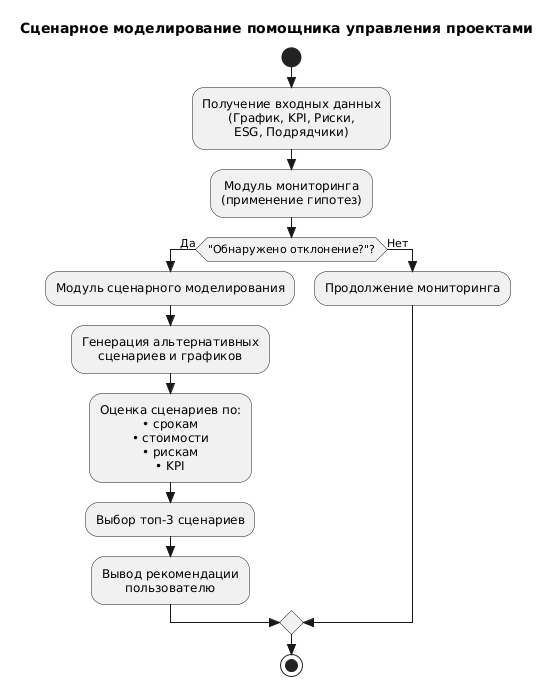
\includegraphics[width=0.9\textwidth]{1.png}
    \caption{Блок-схема сценарного моделирования проекта}
    \label{fig:scenario-model}
\end{figure}

\subsection{Пример сценария}

\textbf{Условие:} Поставка оборудования задерживается на 2 недели.  
\textbf{Риски:} Отклонение от графика, простой подрядчиков, штрафы.  

\textbf{Сценарии:}
\begin{itemize}
    \item С1: Ускорение следующих этапов за счёт перераспределения ресурсов;
    \item С2: Заказ аналогичного оборудования у резервного поставщика;
    \item С3: Продление сроков на 2 недели с уведомлением заказчика и перерасчётом бюджета.
\end{itemize}

Помощник оценивает каждый сценарий по вероятности успеха, стоимости, влиянию на KPI и предлагает наиболее сбалансированное решение.


% Как будет строиться модель: входные данные, дерево сценариев, альтернативные графики
% Пример: "что будет, если задержится поставка сырья на 2 недели?"

\section{RAG-архитектура интеллектуального помощника}

Retrieval-Augmented Generation (RAG) — это архитектура, при которой модель дополнительно использует внешние документы при генерации ответа. Вместо генерации "из головы", помощник сначала извлекает релевантные данные из базы знаний, и только затем формирует ответ на вопрос.

\subsection{Компоненты архитектуры}

\begin{itemize}
    \item \textbf{Интерфейс пользователя} — текстовое поле или API, куда поступает вопрос.
    \item \textbf{Модуль векторизации} — преобразует вопрос в вектор (с помощью модели типа BERT, SBERT, OpenAI embeddings и т.д.).
    \item \textbf{Векторная база данных} — FAISS, ChromaDB, Weaviate и др. Хранит документы в виде векторов.
    \item \textbf{Механизм поиска (retriever)} — находит наиболее близкие документы к вопросу.
    \item \textbf{Генератор (generator)} — LLM (GPT, Mistral, LLaMA и др.), которая генерирует ответ на основе найденных документов.
\end{itemize}

\subsection{Преимущества подхода}

\begin{itemize}
    \item Ответы опираются на актуальные, проверенные источники (например, отчёты компаний).
    \item Нет необходимости дообучать модель при каждом обновлении данных.
    \item Возможна проверка обоснования ответа (цитирование документа).
    \item Удобно реализуется на практике с помощью LangChain, Haystack или собственного пайплайна.
\end{itemize}

\subsection{Пример работы в контексте проекта}

\textbf{Запрос пользователя:}  
«Какие риски учитывает СИБУР при реализации инвестиционных проектов?»

\textbf{Шаги:}
\begin{enumerate}
    \item Векторизуется запрос.
    \item Из векторной БД извлекается фрагмент из годового отчёта СИБУР, содержащий список рисков.
    \item Генератор LLM формирует ответ:  
    \textit{«СИБУР выделяет следующие ключевые риски: макроэкономический, геополитический, логистический, регуляторный…»}
\end{enumerate}

\subsection{Блок-схема архитектуры}

\begin{center}
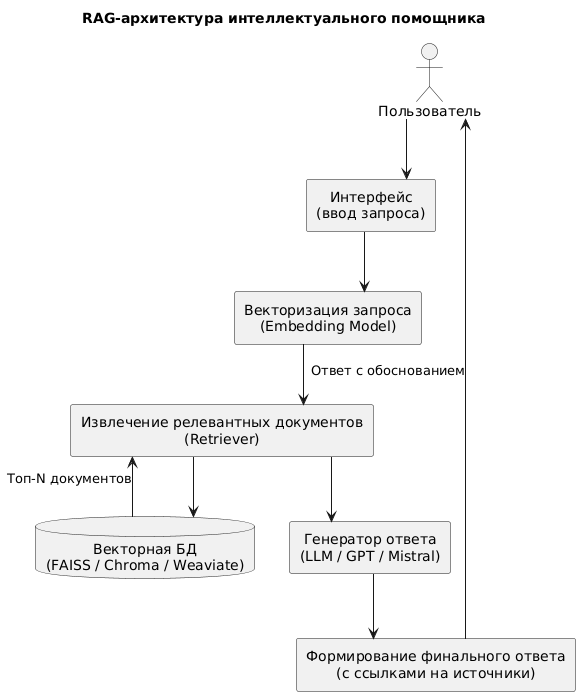
\includegraphics[width=0.85\textwidth]{2.png}
\end{center}


\section{Формирование обучающего датасета для fine-tuning}

Для адаптации языковой модели к контексту управления проектами и специфике российской промышленности подготовлен обучающий набор данных в формате \texttt{jsonl}, содержащий пары «вопрос–ответ» на основе анализа годовых отчётов, внутренних регламентов, сценариев и гипотез мониторинга.

\subsection{Формат данных}

Каждая строка в датасете — это JSON-объект следующего вида:

\begin{lstlisting}
{"prompt": "<question or situation>", "response": "<assistant's response>"}
\end{lstlisting}

\subsection{Примеры обучающих пар}

\begin{lstlisting}
{"prompt": "What are the key risks that SIBUR considers when implementing projects?",
 "response": "SIBUR identifies the following risks: macroeconomic, geopolitical, regulatory, commodity, logistics, and IT risks. Each of these risks is assessed based on its likelihood and impact."}

{"prompt": "Our contractor failed to meet the second consecutive checkpoint. What should we do?",
 "response": "It is recommended to initiate a contractor audit and consider replacing the contractor. This strategy is used in SIBUR's policy. It is also worth recalculating the schedule and assessing the impact on the critical path."}

{"prompt": "The project plan is 17% behind schedule. Should I be concerned?",
 "response": "Yes, according to hypothesis H1, a deviation of more than 15% in terms of time puts the project in the yellow risk zone. It is necessary to analyze the causes and develop corrective measures."}
\end{lstlisting}

\subsection{Источники для генерации обучающего набора}

\begin{itemize}
    \item Годовые и устойчивые отчёты компаний: СИБУР, РОСАТОМ, РУСАЛ;
    \item Внутренние проектные документы и практики;
    \item Гипотезы мониторинга состояния проекта;
    \item Стандартные кейсы: задержки, перерасход бюджета, ESG-отклонения, неустойки, сбои подрядчиков;
    \item Сценарии What-If анализа.
\end{itemize}

\subsection{Объём и требования к датасету}

\begin{itemize}
    \item Количество примеров: от 200 до 2000 строк для начального обучения;
    \item Язык: русский (возможно добавление англ. дублей);
    \item Стиль: нейтральный, деловой, профессиональный;
    \item Допустимые форматы: \texttt{.jsonl}, \texttt{.csv}, \texttt{.xlsx} (для последующей конвертации).
\end{itemize}

\subsection{Используемые модели для fine-tuning}

\begin{itemize}
    \item LLaMA 2 / Mistral / OpenChat;
    \item GPT-3.5-turbo с функцией \texttt{fine-tune} через OpenAI API;
    \item Модели на базе HuggingFace Transformers (например, BERT, Falcon).
\end{itemize}
\subsection{Темы и области охвата обучающего датасета}

Для обеспечения полноты и тематического покрытия обучающего набора данных, все примеры классифицированы по ключевым направлениям. Это позволяет точно адаптировать модель к задачам проектного управления.

\begin{longtable}{|c|p{3.5cm}|p{5.2cm}|p{5.2cm}|}
\hline
\textbf{№} & \textbf{Тема} & \textbf{Примеры вопросов (prompt)} & \textbf{Примеры ответов (response)} \\
\hline
\endfirsthead
\hline
\textbf{№} & \textbf{Тема} & \textbf{Примеры вопросов (prompt)} & \textbf{Примеры ответов (response)} \\
\hline
\endhead

1 & Риски & Какие ключевые риски учитывает СИБУР? \newline Что делать при росте логистических затрат? & Перечисление типов рисков, рекомендации по управлению, ссылка на оценочную модель \\
\hline

2 & Сроки / графики & Сроки отстают на 17\%, что делать? \newline Поставка оборудования задерживается на 2 недели & Генерация сценариев: пересчёт графика, перераспределение задач, использование буферов \\
\hline

3 & Бюджет и стоимость & Проект выходит за бюджет на 12\% \newline Как контролируется CAPEX? & Сценарий перерасчёта бюджета, активизация Value Engineering, уведомление заказчика \\
\hline

4 & KPI & Мы не достигли трёх KPI подряд — это опасно? & Гипотеза H3: система фиксирует угрозу, предлагает анализ и отчёт \\
\hline

5 & ESG / устойчивость & Выбросы CO\textsubscript{2} выросли на 5\% \newline Как проект может попасть в красную зону по ESG? & ESG-триггер, активация сценариев SSP, рекомендации по снижению углеродного следа \\
\hline

6 & Подрядчики & Подрядчик сорвал 2 контрольные точки \newline Как реагировать на подрядчиков с плохой историей? & Анализ контракта, рекомендации по замене, подключение альтернативного исполнителя \\
\hline

7 & ИИ и сбои & Сбой в системе ИИ‑мониторинга качества \newline Что делать при недостоверных данных? & Остановка операций, переход на ручной режим, уведомление руководства \\
\hline

\end{longtable}


\section{Выводы}
Подготовлена концепция интеллектуального помощника, включающего в себя механизм анализа рисков, генерации сценариев, базу знаний по корпоративным практикам и технологическую архитектуру на базе RAG-подхода. Следующим шагом может быть реализация MVP-версии.

\end{document}
